\documentclass[tikz,border=1pt]{standalone}
\usetikzlibrary{tqft,calc}

\begin{document}
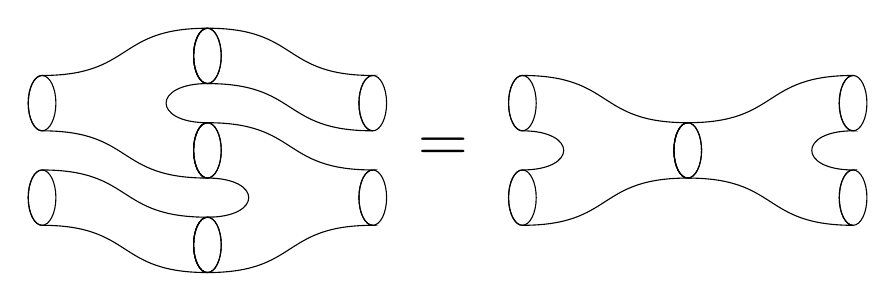
\begin{tikzpicture}[
  % --- global tqft styling (outline-only, like your figure)
  tqft/cobordism/.style={draw},
  tqft/every upper boundary component/.style={draw},
  tqft/every lower boundary component/.style={draw},
  % IMPORTANT: rotate/scale should affect boundary circles too
  every tqft/.style={transform shape},
  % spacing/scale knobs (tune if desired)
  tqft/cobordism height=2.1cm,
  tqft/boundary separation=1.2cm,
]

%========================
% Left-hand side diagram
% (a composite producing 3 seam circles in the middle)
%========================
\begin{scope}[xshift=0cm, yshift=1.2cm]
    \pic[
        tqft/cylinder to prior,
        name=idR,
        rotate=90,
        anchor=incoming boundary 1,
        at={(0,0)}
    ];

    % bottom seam position = one boundary-separation below mu incoming 1
    \coordinate (seamBot) at ($(idR-incoming boundary 1)+(0,-1.2cm)$);
    
    % Second stage: (m ⊔ id)
    \pic[
        tqft/reverse pair of pants,
        name=mu,
        rotate=90,
        anchor=incoming boundary 2,
        at={(seamBot)}
    ];
    
    % First stage: (Δ ⊔ id)
    \pic[
        tqft/pair of pants,
        name=delta,
        rotate=90,
        anchor=outgoing boundary 2,
        at={(idR-incoming boundary 1)}
    ];
    
    \pic[
        tqft/cylinder to prior,
        name=idL,
        rotate=90,
        anchor=outgoing boundary 1,
        at={($(seamBot)+(0,-1.2cm)$)}
    ];
      
\end{scope}

% Equals sign
\node[font=\Huge] at (3,0) {$=$};

%========================
% Right-hand side diagram
% (reverse pants then pants, giving one seam circle)
%========================
\begin{scope}[xshift=4.0cm, yshift=-0.6cm]
  \pic[
    tqft/reverse pair of pants,
    name=m,
    rotate=90
  ];
  \pic[
    tqft/pair of pants,
    name=d,
    rotate=90,
    anchor=incoming boundary 1,
    at=(m-outgoing boundary 1)
  ];
\end{scope}

\end{tikzpicture}
\end{document}